\documentclass[12pt]{article}
\usepackage[a4paper, inner=1.5cm, outer=3cm, top=2cm,bottom=3cm, bindingoffset=1cm]{geometry}
\usepackage[english]{babel}
\usepackage[utf8x]{inputenc}
\usepackage{amsmath}
\usepackage{tikz}
\usepackage{booktabs}
\usepackage{graphicx}
\usepackage{hyperref}
\usepackage{pdflscape}
\usepackage{adjustbox}
\graphicspath{ {./images/} }
\usepackage{capt-of} 
\usepackage{listings}
\usepackage{xcolor}
\usepackage{setspace}
\definecolor{codegreen}{rgb}{0,0.6,0}
\definecolor{codegray}{rgb}{0.5,0.5,0.5}
\definecolor{codepurple}{rgb}{0.58,0,0.82}
\definecolor{backcolour}{rgb}{0.95,0.95,0.92}
 
\lstdefinestyle{mystyle}{
    backgroundcolor=\color{backcolour},   
    commentstyle=\color{codegreen},
    keywordstyle=\color{magenta},
    numberstyle=\tiny\color{codegray},
    stringstyle=\color{codepurple},
    basicstyle=\ttfamily\footnotesize,
    breakatwhitespace=false,         
    breaklines=true,                 
    captionpos=b,                    
    keepspaces=true,                 
    numbers=left,                    
    numbersep=5pt,                  
    showspaces=false,                
    showstringspaces=false,
    showtabs=false,                  
    tabsize=2
}
 
\lstset{style=mystyle}
 
\begin{document}
\begin{titlepage}
\newcommand{\HRule}{\rule{\linewidth}{0.5mm}} 
\center
\doublespacing
\textbf{\Huge MACHINE LEARNING FOR PREDICTING DIABETES MELLITUS}
\\
\singlespacing
\Large
\vspace{3cm}
A project report submitted in partial fulfilment of the requirement for the degree of\\
\vspace{1cm}
\textbf{Bachelor in Science\\In\\Computer Science}
\\by\\
\Large
Alexander Roque Rodrigues
\\
\vspace{1cm}
under the supervision of
\vspace{1cm}
\\
Ashweta Fondekar
\\
\textbf{PARVATIBAI CHOWGULE COLLEGE OF ARTS \& SCIENCE AUTONOMOUS}
\\June 2019
\end{titlepage}

%declaration
\newpage
\vspace{5cm}
\begin{center}

\textbf{Declaration by Candidate}\\

I declare that this project report has been prepared by me and to the best of my
knowledge, it has not previously formed the basis for the award of any diploma or degree by
any other University.



\end{center}
\newpage
CERTIFICATE BY SUPERVISOR\\
Certified that the Project Report is a record of work done by the candidate
himself/herself/themselves under my guidance during the period of study and that to the
best of my knowledge, it has not previously formed the basis of the award of any degree or
diploma of any other University.\\

Ashweta Fondekar\\

Project Supervisor
\newpage

\textbf{Work Record}

\newpage
\section{Acknowledgements}

\newpage
\tableofcontents
\newpage
\listoffigures
\newpage
\listoftables
\newpage


\begin{abstract}

\end{abstract}
\onehalfspacing
%\doublespacing
\section{Introduction}
In recent days, there has been a sharp increase in the cases of diabetes mellitus. Diabetes mellitus is on the rise amongst many people and the rate of contracting this lifestyle disease could be reduced significantly if proper measures and precautions were to be instilled amongst people the number of people can be reduced.

Machine learning is a growing field in computer science. With the development and introduction of many algorithms the prediction and accuracy of the predictions itself has improved substantially. Machine learning and healthcare systems are also becoming increasingly popular in the healthcare sector.

The project encompasses the qualities of Remote Patient Monitoring (RPM) and Clinical Decision Support (CDS). RPM provides medical facilities that have the ability to transmit patient data to healthcare professionals who might very well be halfway around the world. RPM can monitor blood glucose levels and blood pressure. It is particularly helpful for patients with chronic conditions such as type 2 diabetes, hypertension, or cardiac disease. Data collected and transmitted via PRM can be used by a healthcare professional or a healthcare team to detect medical events such as stroke or heart attack that require immediate and aggressive medical intervention. Data collected may be used as part of a research project or health study. RPM is a life-saving system for patients in remote areas who cannot access face-to-face health care. CDS analyzes data from clinical and administrative systems. The aim is to assist healthcare providers in making informed clinical decisions. Data available can provide information to medical professions who are preparing diagnoses or predicting medical conditions like drug interactions and reactions. CDS tools filter information to assist healthcare professionals in caring for individual clients. 

The objective of this project is to create a  system that is able to use the machine learning algorithms and predict the outcome of the parameters entered into the algorithm and help the patient draw a conclusion whether or not he/she has the same traits exhibited by similar patients that have diabetes. Also the system should have a UI that is capable of displaying the data of the patients to the doctor and to the patients themselves for further interpretation.

\newpage
\section{Software Requirements}
The main function of this project is to enable the doctors to advise their patients with the help of the prediction software. The system should be accessible to the patient as well as the doctor, therefore it should have a web interface for the two parties to interact with. 

\subsection{Functionalities for Doctors}
As an owner of a doctors account a doctor should be able to:
\begin{itemize}
\item Add new observations for the machine learning algorithm to predict.
\item Analyse the patients previous records.
\end{itemize}

\subsection{Functionalities for Patients}
As the patient, one should be able to:
\begin{itemize}
\item Should be able to see the predicted risk of developing diabetes.
\item Should be able to view historic data.
\item Should be able to view notes or suggestions left by doctor.
\end{itemize}

\subsection{Functionalities for Master Nodes}
As the master nodes:
\begin{itemize}
\item Control chunk size.
\item Remotely update the slave nodes.
\item Check the availability of nodes.
\item Control the SQL database.
\end{itemize}

\subsection{Functionalities for Slave Nodes}
\begin{itemize}
\item should have the machine learning algorithm with can be updated.
\item Remote access should be possible.
\end{itemize}

\newpage
\section{Hardware Requirements}
\subsection{Raspberry Pi}

According to raspberrypi.org, the Raspberry Pi 3 Model B is the earliest model of the third-generation Raspberry Pi. It replaced the Raspberry Pi 2 Model B in February 2016. Some of the key features of this single board computer or SBC are:
\begin{itemize}
\item Quad Core 1.2GHz Broadcom BCM2837 64bit CPU.
\item 1GB RAM.
\item BCM43438 wireless LAN and Bluetooth Low Energy (BLE) on board.
\item 100 Base Ethernet.
\item 40-pin extended GPIO.
\item 4 USB 2 ports.
\item Full size HDMI.
\item Micro SD port for loading the operating system and storing data.
\end{itemize}
In this project I will be using 3 Raspberry Pi's to implement a cluster and deploy the machine learning algorithm on.

\subsection{Switch}
A network switch was used in the project to make up for the lack of ethernet ports available on the router. The dumb network switch 
was able to connect up-to 3 Raspberry Pi and one cable back to the network router itself to connect the switch to the main network.

\subsection{Router}
A router is required to assign internet protocol addresses to the nodes using dynamic host control protocol (DHCP). The router also is responsible for displaying the nodes connected to the network thereby displaying host names and making it more easier to capture the addresses of each node.

\subsection{Master Node}
The master node is assigned the task of managing the the slave nodes connected to the network. The master node and the slave nodes should be connected to the same database to run and execute queries. The master node shall also be assigned with the task of killing a particular process or shutting down a particular node if required.

\subsection{Slave Node}
The slave nodes are to be configured with the selected algorithm and are the most vital part of the structure. The slave nodes will be responsible for receiving instructions from the master node and will be responsible for learning from the dataset and then can generate predicted outcomes for the patient records received from the master. 

\subsection{Database}
The database will store all the records for the patients and doctors. The database is a SQL database that will not be subjected to a change in the database schema structure for consistency.

\subsection{Web Server}
The web server provides an interface for the doctor and the patients to read the predictions and legacy data of the patient from the website.

\newpage
\section{Technology Stack}
\subsection{Python}
\subsubsection{Pandas}
Pandas, is a library that is required for loading the comma separated value file into python. Pandas is a package for data manipulation and analysis. In particular, it offers data structures and operations for manipulating numerical tables and time series.

\subsubsection{Sklearn}
Scikit-learn is a free software machine learning library for the Python programming language. It features various classification, regression and clustering algorithms including support vector machines, random forests, gradient boosting, k-means and DBSCAN, and is designed to inter-operate with the Python numerical and scientific libraries NumPy and SciPy.

\subsubsection{Numpy}
NumPy is a library for the Python programming language, adding support for large, multi-dimensional arrays and matrices, along with a large collection of high-level mathematical functions to operate on these arrays. The ancestor of NumPy, Numeric, was originally created by Jim Hugunin with contributions from several other developers. In 2005, Travis Oliphant created NumPy by incorporating features of the competing Numarray into Numeric, with extensive modifications. NumPy is open-source software and has many contributors.

\subsubsection{Itertools}
The module standardizes a core set of fast, memory efficient tools that are useful by themselves or in combination. Together, they form an “iterator algebra” making it possible to construct specialized tools succinctly and efficiently in pure Python.

\subsection{MYSQL}
MySQL is an open-source relational database management system (RDBMS). Its name is a combination of "My", the name of co-founder Michael Widenius's daughter, and "SQL", the abbreviation for Structured Query Language.

MySQL is free and open-source software under the terms of the GNU General Public License, and is also available under a variety of proprietary licenses. MySQL was owned and sponsored by the Swedish company MySQL AB, which was bought by Sun Microsystems (now Oracle Corporation). In 2010, when Oracle acquired Sun, Widenius forked the open-source MySQL project to create MariaDB.

MySQL is a component of the LAMP web application software stack (and others), which is an acronym for Linux, Apache, MySQL, Perl/PHP/Python. MySQL is used by many database-driven web applications, including Drupal, Joomla, phpBB, and WordPress. MySQL is also used by many popular websites, including Facebook, Flickr, MediaWiki, Twitter and YouTube.

\subsection{Apache Web Server}
The Apache HTTP Server, colloquially called Apache, is free and open-source cross-platform web server software, released under the terms of Apache License 2.0. Apache is developed and maintained by an open community of developers under the auspices of the Apache Software Foundation.

The vast majority of Apache HTTP Server instances run on a Linux distribution, but current versions also run on Microsoft Windows and a wide variety of Unix-like systems. Past versions also ran on OpenVMS, NetWare, OS/2 and other operating systems, including ports to mainframes.

\subsection{PHP}
PHP is a general-purpose programming language originally designed for web development. PHP originally stood for Personal Home Page,
but it now stands for the recursive initialism PHP: Hypertext Preprocessor.

PHP code may be executed with a command line interface (CLI), embedded into HTML code, or used in combination with various web template systems, web content management systems, and web frameworks. PHP code is usually processed by a PHP interpreter implemented as a module in a web server or as a Common Gateway Interface (CGI) executable. The web server outputs the results of the interpreted and executed PHP code, which may be any type of data, such as generated HTML code or binary image data. PHP can be used for many programming tasks outside of the web context, such as standalone graphical applications and robotic drone control.

\subsection{AJAX}
Ajax is a set of web development techniques using many web technologies on the client side to create asynchronous web applications. With Ajax, web applications can send and retrieve data from a server asynchronously (in the background) without interfering with the display and behavior of the existing page. By decoupling the data interchange layer from the presentation layer, Ajax allows web pages and, by extension, web applications, to change content dynamically without the need to reload the entire page.[3] In practice, modern implementations commonly utilize JSON instead of XML.

Ajax is not a single technology, but rather a group of technologies. HTML and CSS can be used in combination to mark up and style information. The webpage can then be modified by JavaScript to dynamically display—and allow the user to interact with—the new information. The built-in XMLHttpRequest object, or since 2017 the new "fetch()" function within JavaScript, is commonly used to execute Ajax on web pages allowing websites to load content onto the screen without refreshing the page. Ajax is not a new technology, or different language, just existing technologies used in new ways.

\subsection{GitHub}
GitHub is a global company that provides hosting for software development version control using Git. It offers all of the distributed version control and source code management (SCM) functionality of Git as well as adding its own features. It provides access control and several collaboration features such as bug tracking, feature requests, task management, and wikis for every project.

\subsection{SSH}
Secure Shell is a cryptography network protocol for operating network services securely over an unsecured network. Typical applications include remote command-line, login, and remote command execution, but any network service can be secured with SSH. The SSH is used to communicate between the master and slave nodes.

\newpage
\section{Selecting an Algorithm}
% Write about the EDA and algorithm selection process.
The dataset used for this project is from the UCI Machine learning repository and can be found at their website. Table \ref{table:2} is an outcome of the accuracy of the algorithms subjected to train and predict the outcomes for given sets of patients. 

\newpage
\section{The Multi Layered Perceptron}
\subsection{Introduction}
The multi layer perceptron (MLP) is the one of the most commonly used artificial neural networks. The name is a slight misnomer; a multilayer perceptron is not a single perceptron with multiple layers, but rather multiple layers of artificial neurons
that can be perceptrons. The layers of the MLP form a directed, acyclic graph. Generally, each layer is fully connected to the subsequent layer; the output of each artificial neuron in a layer is an input to every artificial neuron in the next layer
towards the output. MLPs have three or more layers of artificial neurons.

\newpage
\section{Coding Process}
% Describe the coding process; write pseudocode; and include images.
The concept of the system remains simple. The system can be described using the following diagrams.
\subsection{Designing the System}
\begin{itemize}

\item The system firstly reads the records from the database that are not classified as 0 or 1. The master node then converts all the results obtained from the database into chunks as specified by the code. 
%step 1 start
\tikzset{every picture/.style={line width=0.75pt}} %set default line width to 0.75pt        
\begin{figure}[!h]
\centering
\begin{tikzpicture}[x=0.75pt,y=0.75pt,yscale=-1,xscale=1]
%uncomment if require: \path (0,300); %set diagram left start at 0, and has height of 300

%Shape: Can [id:dp3989446731507247] 
\draw   (606,68.75) -- (606,170.25) .. controls (606,182.26) and (573.09,192) .. (532.5,192) .. controls (491.91,192) and (459,182.26) .. (459,170.25) -- (459,68.75) .. controls (459,56.74) and (491.91,47) .. (532.5,47) .. controls (573.09,47) and (606,56.74) .. (606,68.75) .. controls (606,80.76) and (573.09,90.5) .. (532.5,90.5) .. controls (491.91,90.5) and (459,80.76) .. (459,68.75) ;
%Shape: Rectangle [id:dp14170681543352437] 
\draw   (102,89) -- (325,89) -- (325,158) -- (102,158) -- cycle ;
%Straight Lines [id:da9571038146445507] 
\draw    (458,121) -- (326.5,121) ;
\draw [shift={(324.5,121)}, rotate = 360] [color={rgb, 255:red, 0; green, 0; blue, 0 }  ][line width=0.75]    (10.93,-3.29) .. controls (6.95,-1.4) and (3.31,-0.3) .. (0,0) .. controls (3.31,0.3) and (6.95,1.4) .. (10.93,3.29)   ;


% Text Node
\draw (213.5,123.5) node   [align=left] {Master Node};
% Text Node
\draw (534,129) node   [align=left] {SQL Database};


\end{tikzpicture}
\caption{Master Node reading data from the SQL Database.}
\end{figure}
%step 1 end

\item odei
%Step 2 start
\tikzset{every picture/.style={line width=0.75pt}} %set default line width to 0.75pt        
\begin{figure}[!h]
\centering

\tikzset{every picture/.style={line width=0.75pt}} %set default line width to 0.75pt        

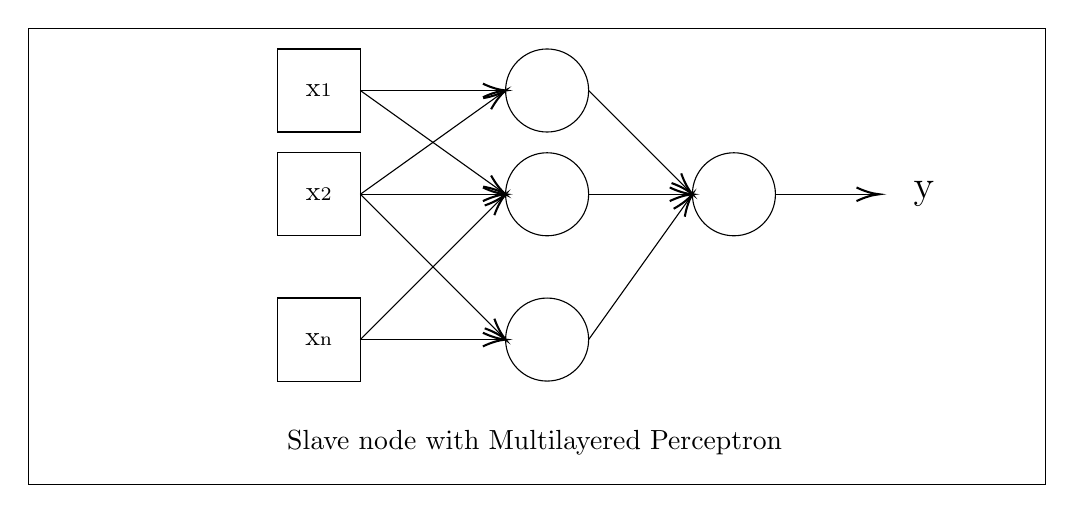
\begin{tikzpicture}[x=0.75pt,y=0.75pt,yscale=-1,xscale=1]
%uncomment if require: \path (0,300); %set diagram left start at 0, and has height of 300

%Shape: Rectangle [id:dp3356543770553979] 
\draw   (70,30) -- (560,30) -- (560,250) -- (70,250) -- cycle ;
%Shape: Square [id:dp5256435827897643] 
\draw   (190,40) -- (230,40) -- (230,80) -- (190,80) -- cycle ;
%Shape: Square [id:dp5270357160077517] 
\draw   (190,90) -- (230,90) -- (230,130) -- (190,130) -- cycle ;
%Shape: Square [id:dp06437153710385335] 
\draw   (190,160) -- (230,160) -- (230,200) -- (190,200) -- cycle ;
%Shape: Circle [id:dp6202571690827927] 
\draw   (300,60) .. controls (300,48.95) and (308.95,40) .. (320,40) .. controls (331.05,40) and (340,48.95) .. (340,60) .. controls (340,71.05) and (331.05,80) .. (320,80) .. controls (308.95,80) and (300,71.05) .. (300,60) -- cycle ;
%Shape: Circle [id:dp7260170908934287] 
\draw   (300,110) .. controls (300,98.95) and (308.95,90) .. (320,90) .. controls (331.05,90) and (340,98.95) .. (340,110) .. controls (340,121.05) and (331.05,130) .. (320,130) .. controls (308.95,130) and (300,121.05) .. (300,110) -- cycle ;
%Shape: Circle [id:dp9546670114782507] 
\draw   (300,180) .. controls (300,168.95) and (308.95,160) .. (320,160) .. controls (331.05,160) and (340,168.95) .. (340,180) .. controls (340,191.05) and (331.05,200) .. (320,200) .. controls (308.95,200) and (300,191.05) .. (300,180) -- cycle ;
%Shape: Circle [id:dp8873752821258001] 
\draw   (390,110) .. controls (390,98.95) and (398.95,90) .. (410,90) .. controls (421.05,90) and (430,98.95) .. (430,110) .. controls (430,121.05) and (421.05,130) .. (410,130) .. controls (398.95,130) and (390,121.05) .. (390,110) -- cycle ;
%Straight Lines [id:da6624191220110807] 
\draw    (230,60) -- (298,60) ;
\draw [shift={(300,60)}, rotate = 180] [color={rgb, 255:red, 0; green, 0; blue, 0 }  ][line width=0.75]    (10.93,-3.29) .. controls (6.95,-1.4) and (3.31,-0.3) .. (0,0) .. controls (3.31,0.3) and (6.95,1.4) .. (10.93,3.29)   ;
%Straight Lines [id:da0866384249373997] 
\draw    (230,110) -- (298,110) ;
\draw [shift={(300,110)}, rotate = 180] [color={rgb, 255:red, 0; green, 0; blue, 0 }  ][line width=0.75]    (10.93,-3.29) .. controls (6.95,-1.4) and (3.31,-0.3) .. (0,0) .. controls (3.31,0.3) and (6.95,1.4) .. (10.93,3.29)   ;
%Straight Lines [id:da13965027003077846] 
\draw    (230,180) -- (298,180) ;
\draw [shift={(300,180)}, rotate = 180] [color={rgb, 255:red, 0; green, 0; blue, 0 }  ][line width=0.75]    (10.93,-3.29) .. controls (6.95,-1.4) and (3.31,-0.3) .. (0,0) .. controls (3.31,0.3) and (6.95,1.4) .. (10.93,3.29)   ;
%Straight Lines [id:da7863905838920622] 
\draw    (230,60) -- (298.37,108.84) ;
\draw [shift={(300,110)}, rotate = 215.54] [color={rgb, 255:red, 0; green, 0; blue, 0 }  ][line width=0.75]    (10.93,-3.29) .. controls (6.95,-1.4) and (3.31,-0.3) .. (0,0) .. controls (3.31,0.3) and (6.95,1.4) .. (10.93,3.29)   ;
%Straight Lines [id:da16736595128940945] 
\draw    (230,110) -- (298.59,178.59) ;
\draw [shift={(300,180)}, rotate = 225] [color={rgb, 255:red, 0; green, 0; blue, 0 }  ][line width=0.75]    (10.93,-3.29) .. controls (6.95,-1.4) and (3.31,-0.3) .. (0,0) .. controls (3.31,0.3) and (6.95,1.4) .. (10.93,3.29)   ;
%Straight Lines [id:da837081391568496] 
\draw    (230,180) -- (298.59,111.41) ;
\draw [shift={(300,110)}, rotate = 495] [color={rgb, 255:red, 0; green, 0; blue, 0 }  ][line width=0.75]    (10.93,-3.29) .. controls (6.95,-1.4) and (3.31,-0.3) .. (0,0) .. controls (3.31,0.3) and (6.95,1.4) .. (10.93,3.29)   ;
%Straight Lines [id:da0751297016521475] 
\draw    (230,110) -- (298.37,61.16) ;
\draw [shift={(300,60)}, rotate = 504.46] [color={rgb, 255:red, 0; green, 0; blue, 0 }  ][line width=0.75]    (10.93,-3.29) .. controls (6.95,-1.4) and (3.31,-0.3) .. (0,0) .. controls (3.31,0.3) and (6.95,1.4) .. (10.93,3.29)   ;
%Straight Lines [id:da2549769311708434] 
\draw    (340,180) -- (388.84,111.63) ;
\draw [shift={(390,110)}, rotate = 485.54] [color={rgb, 255:red, 0; green, 0; blue, 0 }  ][line width=0.75]    (10.93,-3.29) .. controls (6.95,-1.4) and (3.31,-0.3) .. (0,0) .. controls (3.31,0.3) and (6.95,1.4) .. (10.93,3.29)   ;
%Straight Lines [id:da5966427506538203] 
\draw    (340,110) -- (388,110) ;
\draw [shift={(390,110)}, rotate = 180] [color={rgb, 255:red, 0; green, 0; blue, 0 }  ][line width=0.75]    (10.93,-3.29) .. controls (6.95,-1.4) and (3.31,-0.3) .. (0,0) .. controls (3.31,0.3) and (6.95,1.4) .. (10.93,3.29)   ;
%Straight Lines [id:da30294544760077824] 
\draw    (340,60) -- (388.59,108.59) ;
\draw [shift={(390,110)}, rotate = 225] [color={rgb, 255:red, 0; green, 0; blue, 0 }  ][line width=0.75]    (10.93,-3.29) .. controls (6.95,-1.4) and (3.31,-0.3) .. (0,0) .. controls (3.31,0.3) and (6.95,1.4) .. (10.93,3.29)   ;
%Straight Lines [id:da77593748506778] 
\draw    (430,110) -- (478,110) ;
\draw [shift={(480,110)}, rotate = 180] [color={rgb, 255:red, 0; green, 0; blue, 0 }  ][line width=0.75]    (10.93,-3.29) .. controls (6.95,-1.4) and (3.31,-0.3) .. (0,0) .. controls (3.31,0.3) and (6.95,1.4) .. (10.93,3.29)   ;

% Text Node
\draw (314,229.5) node   [align=left] {Slave node with Multilayered Perceptron};
% Text Node
\draw (210,60) node   [align=left] {x{\scriptsize 1}};
% Text Node
\draw (210,110) node   [align=left] {x{\scriptsize 2}};
% Text Node
\draw (210,180) node   [align=left] {x{\scriptsize n}};
% Text Node
\draw (501.5,110) node   [align=left] {{\Large y}};


\end{tikzpicture}
\end{figure}
%Step 2 end

\newpage
\item The chunks containing the data of the queries that were left unpredicted via the cluster are sent to the cluster in a round robin fashion. The 
%step 3

\tikzset{every picture/.style={line width=0.75pt}} %set default line width to 0.75pt        
\begin{figure}[!h]
\centering
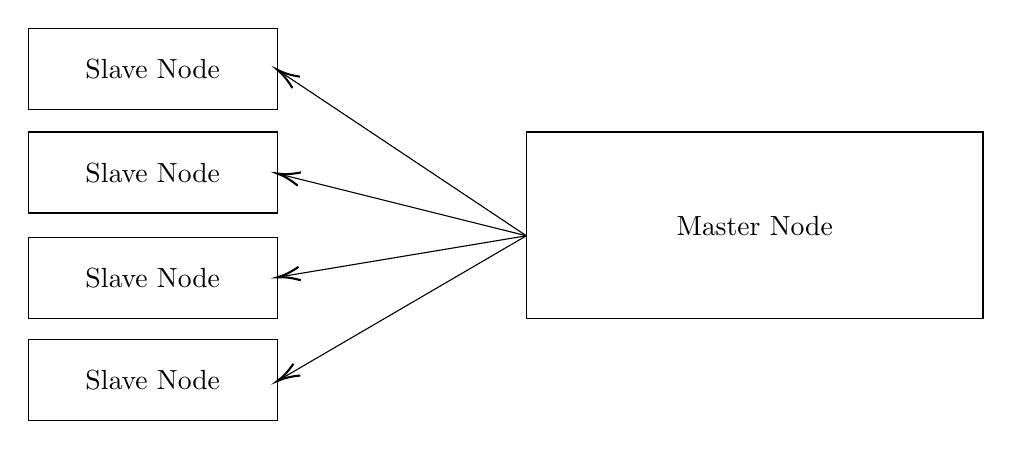
\begin{tikzpicture}[x=0.75pt,y=0.75pt,yscale=-1,xscale=1]
%uncomment if require: \path (0,300); %set diagram left start at 0, and has height of 300

%Shape: Rectangle [id:dp7056891731575645] 
\draw   (100,151) -- (220,151) -- (220,190) -- (100,190) -- cycle ;
%Shape: Rectangle [id:dp652502983568856] 
\draw   (100,200) -- (220,200) -- (220,239) -- (100,239) -- cycle ;
%Shape: Rectangle [id:dp1370792081503991] 
\draw   (100,50) -- (220,50) -- (220,89) -- (100,89) -- cycle ;
%Shape: Rectangle [id:dp3403063589466713] 
\draw   (100,100) -- (220,100) -- (220,139) -- (100,139) -- cycle ;
%Shape: Rectangle [id:dp05437739213565784] 
\draw   (340,100) -- (560,100) -- (560,190) -- (340,190) -- cycle ;
%Straight Lines [id:da17081303413935167] 
\draw    (340,150) -- (221.66,71.11) ;
\draw [shift={(220,70)}, rotate = 393.69] [color={rgb, 255:red, 0; green, 0; blue, 0 }  ][line width=0.75]    (10.93,-3.29) .. controls (6.95,-1.4) and (3.31,-0.3) .. (0,0) .. controls (3.31,0.3) and (6.95,1.4) .. (10.93,3.29)   ;
%Straight Lines [id:da6256697337377781] 
\draw    (340,150) -- (221.94,120.49) ;
\draw [shift={(220,120)}, rotate = 374.03999999999996] [color={rgb, 255:red, 0; green, 0; blue, 0 }  ][line width=0.75]    (10.93,-3.29) .. controls (6.95,-1.4) and (3.31,-0.3) .. (0,0) .. controls (3.31,0.3) and (6.95,1.4) .. (10.93,3.29)   ;
%Straight Lines [id:da3463514586442602] 
\draw    (340,150) -- (221.97,169.67) ;
\draw [shift={(220,170)}, rotate = 350.53999999999996] [color={rgb, 255:red, 0; green, 0; blue, 0 }  ][line width=0.75]    (10.93,-3.29) .. controls (6.95,-1.4) and (3.31,-0.3) .. (0,0) .. controls (3.31,0.3) and (6.95,1.4) .. (10.93,3.29)   ;
%Straight Lines [id:da6887749797140261] 
\draw    (340,150) -- (221.73,218.99) ;
\draw [shift={(220,220)}, rotate = 329.74] [color={rgb, 255:red, 0; green, 0; blue, 0 }  ][line width=0.75]    (10.93,-3.29) .. controls (6.95,-1.4) and (3.31,-0.3) .. (0,0) .. controls (3.31,0.3) and (6.95,1.4) .. (10.93,3.29)   ;

% Text Node
\draw (160,170.5) node   [align=left] {Slave Node};
% Text Node
\draw (160,219.5) node   [align=left] {Slave Node};
% Text Node
\draw (160,119.5) node   [align=left] {Slave Node};
% Text Node
\draw (160,69.5) node   [align=left] {Slave Node};
% Text Node
\draw (450,145) node   [align=left] {Master Node};


\end{tikzpicture}
\end{figure}

%step 3 end

\end{itemize}
\clearpage
\newpage
\section{Deploying to Cluster}
A cluster is a group of two or more servers connected to each other in such a way that they behave like a single server. Each machine in the cluster is called a node. Because each machine in the cluster runs the same services as other machines in the cluster, any machine can stand in for any other machine in the cluster. This becomes important when one machine goes down or must be taken out of service for a time. The remaining machines in the cluster can seamlessly take over the work of the downed machine, providing users with uninterrupted access to services and data.

Benefits of Clustering
Clustering Intelligence Servers provides the following benefits:

Increased resource availability: If one Intelligence Server in a cluster fails, the other Intelligence Servers in the cluster can pick up the workload. This prevents the loss of valuable time and information if a server fails.
Strategic resource usage: You can distribute projects across nodes in whatever configuration you prefer. This reduces overhead because not all machines need to be running all projects, and allows you to use your resources flexibly.
Increased performance: Multiple machines provide greater processing power.
Greater scalability: As your user base grows and report complexity increases, your resources can grow.
Simplified management: Clustering simplifies the management of large or rapidly growing systems.
Fail-over Support
Fail-over support ensures that a business intelligence system remains available for use if an application or hardware failure occurs. Clustering provides failover support in two ways:

Load redistribution: When a node fails, the work for which it is responsible is directed to another node or set of nodes.
Request recovery: When a node fails, the system attempts to reconnect MicroStrategy Web users with queued or processing requests to another node. Users must log in again to be authenticated on the new node. The user is prompted to resubmit job requests.
Load Balancing
Load balancing is a strategy aimed at achieving even distribution of user sessions across Intelligence Servers, so that no single machine is overwhelmed. This strategy is especially valuable when it is difficult to predict the number of requests a server will receive. MicroStrategy achieves four-tier load balancing by incorporating load balancers into the MicroStrategy Web and Web products.

Load is calculated as the number of user sessions connected to a node. The load balancers collect information on the number of user sessions each node is carrying. Using this information at the time a user logs in to a project, MicroStrategy Web connects them to the Intelligence Server node that is carrying the lightest session load. All requests by that user are routed to the node to which they are connected until the user disconnects from the MicroStrategy Web product.

Project Distribution and Project Fail over
When you set up several server machines in a cluster, you can distribute projects across those clustered machines or nodes in any configuration, in both Windows and Linux environments. All servers in a cluster do not need to be running all projects. Each node in the cluster can host a different set of projects, which means only a subset of projects need to be loaded on a specific Intelligence Server machine. This feature provides you with flexibility in using your resources, and it provides better scalability and performance because of less overhead on each Intelligence Server machine.

Distributing projects across nodes also provides project fail-over support. For example, one server is hosting project A and another server is hosting projects B and C. If the first server fails, the other server can host all three projects to ensure project availability.

Project creation, duplication, and deletion in a three-tier, or server, connection are automatically broadcast to all nodes during run-time to ensure synchronization across the cluster.

Work Fencing
User fences and workload fences allow you to reserve nodes of a cluster for either users or a project subscriptions. 

\newpage
\section{Future Scope}

\newpage
\section{Tables}
{
\clearpage
\thispagestyle{empty}
\begin{landscape}
\centering
\begin{table}[]
\centering
\begin{tabular}{|l|l|}
\hline
Column Name                & Description                                                               \\ \hline
Pregnancies                & Number of times pregnant.                                                 \\ \hline
Glucose                    & Plasma glucose concentration a 2 hours in an oral glucose tolerance test. \\ \hline
Blood Pressure             & Diastolic blood pressure (mm Hg)                                          \\ \hline
Skin Thickness             & Triceps skin fold thickness (mm)                                          \\ \hline
Insulin                    & 2-Hour serum insulin (muU/ml)                                            \\ \hline
Body Mass Index            & Body mass index (weight in kg/(height in m)\textasciicircum{}2)           \\ \hline
Diabetes Pedigree Function & Diabetes pedigree function                                                \\ \hline
Age                        & Age (years)                                                               \\ \hline
Outcome                    & Class variable (0 or 1) 268 of 768 are 1, the others are 0                \\ \hline
\end{tabular}
\end{table}
\captionof{table}{Pima Indians dataset header.}
\label{table:1}
\end{landscape}
\clearpage
}


{
\clearpage
\thispagestyle{empty}
\begin{landscape}
\centering
\begin{table}[]
\begin{tabular}{|c|c|c|c|}
\hline
Algorithm              & Additional Parameters                              & Train Set Accuracy & Test Set Accuracy \\ \hline
K Nearest Neighbour    & -                                                  & 0.79               & 0.78              \\ \hline
Logistic Regression    & C = 1                                              & 0.781              & 0.771             \\ \hline
Logistic Regression    & C = 0.01                                           & 0.700              & 0.703             \\ \hline
Logistic Regression    & C = 100                                            & 0.785              & 0.766             \\ \hline
Decision Tree          & -                                                  & 1.00               & 0.714             \\ \hline
Decision Tree          & Max Depth = 3                                      & 0.773              & 0.740             \\ \hline
Random Forest          & Estimators = 100                                   & 1.000              & 0.786             \\ \hline
Random Forest          & Estimators = 100; Max Depth = 3                    & 0.800              & 0.755             \\ \hline
Gradient Boosting      & -                                                  & 0.917              & 0.792             \\ \hline
Gradient Boosting      & Max Depth = 1                                      & 0.804              & 0.781             \\ \hline
Gradient Boosting      & Learning Rate = 0.01                               & 0.802              & 0.776             \\ \hline
Support Vector Machine & -                                                  & 1.00               & 0.65              \\ \hline
Support Vector Machine & Train and Test set scaled using MinMaxScaler       & 0.77               & 0.77              \\ \hline
Support Vector Machine & C = 1000                                           & 0.790              & 0.797             \\ \hline
MLP Classifier         & Random State = 42                                  & 0.73               & 0.72              \\ \hline
MLP Classifier         & Random State = 0                                   & 0.823              & 0.802             \\ \hline
MLP Classifier         & Max Iterations = 1000                              & 0.908              & 0.792             \\ \hline
MLP Classifier         & Max Iterations = 1000; Alpha = 1; Random State = 0 & 0.806              & 0.797             \\ \hline
\end{tabular}
\end{table}
\captionof{table}{Test and Train accuracy's using various machine learning algorithms with various parameters.}
\label{table:2}
\end{landscape}
\clearpage
}

\newpage
\section{Appendices}
\subsection{K Nearest Neighbours}
\subsubsection{Function Syntax}
\begin{lstlisting}
class sklearn.neighbors.KNeighborsClassifier(n_neighbors=5, weights='uniform', algorithm='auto', leaf_size=30, p=2, metric='minkowski', metric_params=None, n_jobs=None, **kwargs)
\end{lstlisting}

\subsubsection{Parameters}
\begin{itemize}
\item \texttt{n\textunderscore neighbors}`
Number of neighbors to use by default for kneighbors queries.

\item
\texttt{weights}
weight function used in prediction. Possible values:

‘uniform’ : uniform weights. All points in each neighborhood are weighted equally.

‘distance’ : weight points by the inverse of their distance. in this case, closer neighbors of a query point will have a greater influence than neighbors which are further away.

[callable] : a user-defined function which accepts an array of distances, and returns an array of the same shape containing the weights.

\item{algorithm}{‘auto’, ‘ball \textunderscore tree’, ‘kd\textunderscore tree’, ‘brute’}, optional
Algorithm used to compute the nearest neighbors:

‘ball\textunderscore tree’ will use BallTree

‘kd\textunderscore tree’ will use KDTree

‘brute’ will use a brute-force search.

‘auto’ will attempt to decide the most appropriate algorithm based on the values passed to fit method.

Note: fitting on sparse input will override the setting of this parameter, using brute force.

\item \texttt{leaf\textunderscore size }int, optional (default = 30)
Leaf size passed to BallTree or KDTree. This can affect the speed of the construction and query, as well as the memory required to store the tree. The optimal value depends on the nature of the problem.

\item \texttt{p} integer, optional (default = 2)
Power parameter for the Minkowski metric. When p = 1, this is equivalent to using manhattan\textunderscore distance (l1), and euclidean\textunderscore distance (l2) for p = 2. For arbitrary p, minkowski\textunderscore distance (l\textunderscore p) is used.

\item \texttt{metric} string or callable, default ‘minkowski’
the distance metric to use for the tree. The default metric is minkowski, and with p=2 is equivalent to the standard Euclidean metric. See the documentation of the DistanceMetric class for a list of available metrics. If metric is “precomputed”, X is assumed to be a distance matrix and must be square during fit. X may be a Glossary, in which case only “nonzero” elements may be considered neighbors.

\item
metric\textunderscore params dict, optional (default = None)
Additional keyword arguments for the metric function.

\item
n\textunderscore jobsint or None, optional (default=None)
The number of parallel jobs to run for neighbors search. None means 1 unless in a joblib.parallel\textunderscore backend context. -1 means using all processors. See Glossary for more details. Doesn’t affect fit method.
\end{itemize}

\newpage
\subsubsection{Logistic Regression}
\begin{lstlisting}
class sklearn.linear_model.LogisticRegression(penalty='l2', dual=False, tol=0.0001, C=1.0, fit_intercept=True, intercept_scaling=1, class_weight=None, random_state=None, solver='lbfgs', max_iter=100, multi_class='auto', verbose=0, warm_start=False, n_jobs=None, l1_ratio=None)
\end{lstlisting}


\begin{itemize}
\item
penalty{‘l1’, ‘l2’, ‘elasticnet’, ‘none’}, default=’l2’
Used to specify the norm used in the penalization. The ‘newton-cg’, ‘sag’ and ‘lbfgs’ solvers support only l2 penalties. ‘elasticnet’ is only supported by the ‘saga’ solver. If ‘none’ (not supported by the liblinear solver), no regularization is applied.

\item
dualbool, default=False
Dual or primal formulation. Dual formulation is only implemented for l2 penalty with liblinear solver. Prefer dual=False when n\textunderscore samples > n\textunderscore features.

\item
tolfloat, default=1e-4
Tolerance for stopping criteria.

\item
Cfloat, default=1.0
Inverse of regularization strength; must be a positive float. Like in support vector machines, smaller values specify stronger regularization.

\item
fit\textunderscore interceptbool, default=True
Specifies if a constant (a.k.a. bias or intercept) should be added to the decision function.

\item
intercept\textunderscore scalingfloat, default=1
Useful only when the solver ‘liblinear’ is used and self.fit\textunderscore intercept is set to True. 
In this case, x becomes [x, self.intercept\textunderscore scaling], i.e. a “synthetic” feature with constant value equal to intercept\textunderscore scaling is appended to the instance vector. The intercept becomes intercept\textunderscore scaling * synthetic\textunderscore feature\textunderscore weight.


\item
class\textunderscore weightdict or ‘balanced’, default=None
Weights associated with classes in the form {class\textunderscore label: weight}. If not given, all classes are supposed to have weight one.

\item
The “balanced” mode uses the values of y to automatically adjust weights inversely proportional to class frequencies in the input data as n\textunderscore samples / (n\textunderscore classes * np.bincount(y)).

\item
random\textunderscore stateint, RandomState instance, default=None
The seed of the pseudo random number generator to use when shuffling the data. If int, random\textunderscore state is the seed used by the random number generator; If RandomState instance, random\textunderscore state is the random number generator; If None, the random number generator is the RandomState instance used by np.random. Used when solver == ‘sag’ or ‘liblinear’.

\item
solver{‘newton-cg’, ‘lbfgs’, ‘liblinear’, ‘sag’, ‘saga’}, default=’lbfgs’
Algorithm to use in the optimization problem.

For small datasets, ‘liblinear’ is a good choice, whereas ‘sag’ and ‘saga’ are faster for large ones.

For multiclass problems, only ‘newton-cg’, ‘sag’, ‘saga’ and ‘lbfgs’ handle multinomial loss; ‘liblinear’ is limited to one-versus-rest schemes.

‘newton-cg’, ‘lbfgs’, ‘sag’ and ‘saga’ handle L2 or no penalty

‘liblinear’ and ‘saga’ also handle L1 penalty

‘saga’ also supports ‘elasticnet’ penalty

‘liblinear’ does not support setting penalty='none'


\item
max\textunderscore iterint, default=100
Maximum number of iterations taken for the solvers to converge.

\item
multi\textunderscore class{‘auto’, ‘ovr’, ‘multinomial’}, default=’auto’
If the option chosen is ‘ovr’, then a binary problem is fit for each label. For ‘multinomial’ the loss minimised is the multinomial loss fit across the entire probability distribution, even when the data is binary. ‘multinomial’ is unavailable when solver=’liblinear’. ‘auto’ selects ‘ovr’ if the data is binary, or if solver=’liblinear’, and otherwise selects ‘multinomial’.

\item
verboseint, default=0
For the liblinear and lbfgs solvers set verbose to any positive number for verbosity.

\item
warm\textunderscore startbool, default=False
When set to True, reuse the solution of the previous call to fit as initialization, otherwise, just erase the previous solution. Useless for liblinear solver. See the Glossary.

\item
n\textunderscore jobsint, default=None
Number of CPU cores used when parallelizing over classes if multi\textunderscore class=’ovr’”. This parameter is ignored when the solver is set to ‘liblinear’ regardless of whether ‘multi\textunderscore class’ is specified or not. None means 1 unless in a joblib.parallel\textunderscore backend context. -1 means using all processors. See Glossary for more details.

\item
l1\textunderscore ratiofloat, default=None
The Elastic-Net mixing parameter, with 0 <= l1\textunderscore ratio <= 1. Only used if penalty='elasticnet'`. Setting ``l1\textunderscore ratio=0 is equivalent to using penalty='l2', while setting l1\textunderscore ratio=1 is equivalent to using penalty='l1'. For 0 < l1\textunderscore ratio <1, the penalty is a combination of L1 and L2.
\end{itemize}

\subsubsection{Decision Tree}
\begin{lstlisting}
class sklearn.tree.DecisionTreeClassifier(criterion='gini', splitter='best', max_depth=None, min_samples_split=2, min_samples_leaf=1, min_weight_fraction_leaf=0.0, max_features=None, random_state=None, max_leaf_nodes=None, min_impurity_decrease=0.0, min_impurity_split=None, class_weight=None, presort='deprecated', ccp_alpha=0.0)
\end{lstlisting}

\begin{itemize}

\item
criterion{“gini”, “entropy”}, default=”gini”
The function to measure the quality of a split. Supported criteria are “gini” for the Gini impurity and “entropy” for the information gain.

\item
splitter{“best”, “random”}, default=”best”
The strategy used to choose the split at each node. Supported strategies are “best” to choose the best split and “random” to choose the best random split.

\item
max\textunderscore depthint, default=None
The maximum depth of the tree. If None, then nodes are expanded until all leaves are pure or until all leaves contain less than min\textunderscore samples\textunderscore split samples.


\item
min\textunderscore samples\textunderscore splitint or float, default=2
The minimum number of samples required to split an internal node:

If int, then consider min\textunderscore samples\textunderscore split as the minimum number.

If float, then min\textunderscore samples\textunderscore split is a fraction and ceil(min\textunderscore samples\textunderscore split * n\textunderscore samples) are the minimum number of samples for each split.

\item
min\textunderscore samples\textunderscore leafint or float, default=1
The minimum number of samples required to be at a leaf node. A split point at any depth will only be considered if it leaves at least min\textunderscore samples\textunderscore leaf training samples in each of the left and right branches. This may have the effect of smoothing the model, especially in regression.

If int, then consider min\textunderscore samples\textunderscore leaf as the minimum number.

If float, then min\textunderscore samples\textunderscore leaf is a fraction and ceil(min\textunderscore samples\textunderscore leaf * n\textunderscore samples) are the minimum number of samples for each node.

\item
min\textunderscore weight\textunderscore fraction\textunderscore leaffloat, default=0.0
The minimum weighted fraction of the sum total of weights (of all the input samples) required to be at a leaf node. Samples have equal weight when sample\textunderscore weight is not provided.

max\textunderscore featuresint, float or {“auto”, “sqrt”, “log2”}, default=None
The number of features to consider when looking for the best split:

If int, then consider max\textunderscore features features at each split.

If float, then max\textunderscore features is a fraction and int(max\textunderscore features * n\textunderscore features) features are considered at each split.

If “auto”, then max\textunderscore features=sqrt(n\textunderscore features).

If “sqrt”, then max\textunderscore features=sqrt(n\textunderscore features).

If “log2”, then max\textunderscore features=log2(n\textunderscore features).

If None, then max\textunderscore features=n\textunderscore features.

Note: the search for a split does not stop until at least one valid partition of the node samples is found, even if it requires to effectively inspect more than max\textunderscore features features.


\item
random\textunderscore stateint or RandomState, default=None
If int, random\textunderscore state is the seed used by the random number generator; If RandomState instance, random\textunderscore state is the random number generator; If None, the random number generator is the RandomState instance used by np.random.


\item
max\textunderscore leaf\textunderscore nodesint, default=None
Grow a tree with max\textunderscore leaf\textunderscore nodes in best-first fashion. Best nodes are defined as relative reduction in impurity. If None then unlimited number of leaf nodes.

\item
min\textunderscore impurity\textunderscore decreasefloat, default=0.0
A node will be split if this split induces a decrease of the impurity greater than or equal to this value.

\item
ccp\textunderscore alphanon-negative float, default=0.0
Complexity parameter used for Minimal Cost-Complexity Pruning. The subtree with the largest cost complexity that is smaller than ccp\textunderscore alpha will be chosen. By default, no pruning is performed. See Minimal Cost-Complexity Pruning for details.

\end{itemize}

\newpage
\subsubsection{Random Forest Classifier}
\begin{lstlisting}
class sklearn.ensemble.RandomForestClassifier(n_estimators=100, criterion='gini', max_depth=None, min_samples_split=2, min_samples_leaf=1, min_weight_fraction_leaf=0.0, max_features='auto', max_leaf_nodes=None, min_impurity_decrease=0.0, min_impurity_split=None, bootstrap=True, oob_score=False, n_jobs=None, random_state=None, verbose=0, warm_start=False, class_weight=None, ccp_alpha=0.0, max_samples=None)
\end{lstlisting}

\begin{itemize}
\item
n\textunderscore estimatorsinteger, optional (default=100)
The number of trees in the forest.

\item
criterionstring, optional (default=”gini”)
The function to measure the quality of a split. Supported criteria are “gini” for the Gini impurity and “entropy” for the information gain. Note: this parameter is tree-specific.

\item
max\textunderscore depthinteger or None, optional (default=None)
The maximum depth of the tree. If None, then nodes are expanded until all leaves are pure or until all leaves contain less than min\textunderscore samples\textunderscore split samples.

\item
min\textunderscore samples\textunderscore splitint, float, optional (default=2)
The minimum number of samples required to split an internal node:

If int, then consider min\textunderscore samples\textunderscore split as the minimum number.

If float, then min\textunderscore samples\textunderscore split is a fraction and ceil(min\textunderscore samples\textunderscore split * n\textunderscore samples) are the minimum number of samples for each split.

\item
min\textunderscore samples\textunderscore leafint, float, optional (default=1)
The minimum number of samples required to be at a leaf node. A split point at any depth will only be considered if it leaves at least min\textunderscore samples\textunderscore leaf training samples in each of the left and right branches. This may have the effect of smoothing the model, especially in regression.

If int, then consider min\textunderscore samples\textunderscore leaf as the minimum number.

If float, then min\textunderscore samples\textunderscore leaf is a fraction and ceil(min\textunderscore samples\textunderscore leaf * n\textunderscore samples) are the minimum number of samples for each node.

Changed in version 0.18: Added float values for fractions.

\item
min\textunderscore weight\textunderscore fraction\textunderscore leaffloat, optional (default=0.)
The minimum weighted fraction of the sum total of weights (of all the input samples) required to be at a leaf node. Samples have equal weight when sample\textunderscore weight is not provided.

\item
max\textunderscore featuresint, float, string or None, optional (default=”auto”)
The number of features to consider when looking for the best split:

If int, then consider max\textunderscore features features at each split.

If float, then max\textunderscore features is a fraction and int(max\textunderscore features * n\textunderscore features) features are considered at each split.

If “auto”, then max\textunderscore features=sqrt(n\textunderscore features).

If “sqrt”, then max\textunderscore features=sqrt(n\textunderscore features) (same as “auto”).

If “log2”, then max\textunderscore features=log2(n\textunderscore features).

If None, then max\textunderscore features=n\textunderscore features.

Note: the search for a split does not stop until at least one valid partition of the node samples is found, even if it requires to effectively inspect more than max\textunderscore features features.

\item
max\textunderscore leaf\textunderscore nodesint or None, optional (default=None)
Grow trees with max\textunderscore leaf\textunderscore nodes in best-first fashion. Best nodes are defined as relative reduction in impurity. If None then unlimited number of leaf nodes.

\item
min\textunderscore impurity\textunderscore decreasefloat, optional (default=0.)
A node will be split if this split induces a decrease of the impurity greater than or equal to this value.

\item
min\textunderscore impurity\textunderscore splitfloat, (default=1e-7)
Threshold for early stopping in tree growth. A node will split if its impurity is above the threshold, otherwise it is a leaf.

\item
oob\textunderscore scorebool (default=False)
Whether to use out-of-bag samples to estimate the generalization accuracy.

\item
n\textunderscore jobsint or None, optional (default=None)
The number of jobs to run in parallel. fit, predict, decision\textunderscore path and apply are all parallelized over the trees. None means 1 unless in a joblib.parallel\textunderscore backend context. -1 means using all processors. See Glossary for more details.

\item
random\textunderscore stateint, RandomState instance or None, optional (default=None)
Controls both the randomness of the bootstrapping of the samples used when building trees (if bootstrap=True) and the sampling of the features to consider when looking for the best split at each node (if max\textunderscore features < n\textunderscore features). See Glossary for details.

\item
verboseint, optional (default=0)
Controls the verbosity when fitting and predicting.

\item
warm\textunderscore startbool, optional (default=False)
When set to True, reuse the solution of the previous call to fit and add more estimators to the ensemble, otherwise, just fit a whole new forest. See the Glossary.

\item
class\textunderscore weightdict, list of dicts, “balanced”, “balanced\textunderscore subsample” or None, optional (default=None)
Weights associated with classes in the form {class\textunderscore label: weight}. If not given, all classes are supposed to have weight one. For multi-output problems, a list of dicts can be provided in the same order as the columns of y.

\item
ccp\textunderscore alphanon-negative float, optional (default=0.0)
Complexity parameter used for Minimal Cost-Complexity Pruning. The subtree with the largest cost complexity that is smaller than ccp\textunderscore alpha will be chosen. By default, no pruning is performed. See Minimal Cost-Complexity Pruning for details.

\item
max\textunderscore samplesint or float, default=None
If bootstrap is True, the number of samples to draw from X to train each base estimator.

If None (default), then draw X.shape[0] samples.

If int, then draw max\textunderscore samples samples.

If float, then draw max\textunderscore samples * X.shape[0] samples. Thus, max\textunderscore samples should be in the interval (0, 1).

\end{itemize}

\newpage
\subsubsection{Gradient Boosting}
\begin{lstlisting}
class sklearn.ensemble.GradientBoostingClassifier(loss='deviance', learning_rate=0.1, n_estimators=100, subsample=1.0, criterion='friedman_mse', min_samples_split=2, min_samples_leaf=1, min_weight_fraction_leaf=0.0, max_depth=3, min_impurity_decrease=0.0, min_impurity_split=None, init=None, random_state=None, max_features=None, verbose=0, max_leaf_nodes=None, warm_start=False, presort='deprecated', validation_fraction=0.1, n_iter_no_change=None, tol=0.0001, ccp_alpha=0.0)
\end{lstlisting}

\begin{itemize}
\item
loss{‘deviance’, ‘exponential’}, optional (default=’deviance’)
loss function to be optimized. ‘deviance’ refers to deviance (= logistic regression) for classification with probabilistic outputs. For loss ‘exponential’ gradient boosting recovers the AdaBoost algorithm.

learning\textunderscore ratefloat, optional (default=0.1)
learning rate shrinks the contribution of each tree by learning\textunderscore rate. There is a trade-off between learning\textunderscore rate and n\textunderscore estimators.

n\textunderscore estimatorsint (default=100)
The number of boosting stages to perform. Gradient boosting is fairly robust to over-fitting so a large number usually results in better performance.

subsamplefloat, optional (default=1.0)
The fraction of samples to be used for fitting the individual base learners. If smaller than 1.0 this results in Stochastic Gradient Boosting. subsample interacts with the parameter n\textunderscore estimators. Choosing subsample < 1.0 leads to a reduction of variance and an increase in bias.

criterionstring, optional (default=”friedman\textunderscore mse”)
The function to measure the quality of a split. Supported criteria are “friedman\textunderscore mse” for the mean squared error with improvement score by Friedman, “mse” for mean squared error, and “mae” for the mean absolute error. The default value of “friedman\textunderscore mse” is generally the best as it can provide a better approximation in some cases.

New in version 0.18.

min\textunderscore samples\textunderscore splitint, float, optional (default=2)
The minimum number of samples required to split an internal node:

If int, then consider min\textunderscore samples\textunderscore split as the minimum number.

If float, then min\textunderscore samples\textunderscore split is a fraction and ceil(min\textunderscore samples\textunderscore split * n\textunderscore samples) are the minimum number of samples for each split.

Changed in version 0.18: Added float values for fractions.

min\textunderscore samples\textunderscore leafint, float, optional (default=1)
The minimum number of samples required to be at a leaf node. A split point at any depth will only be considered if it leaves at least min\textunderscore samples\textunderscore leaf training samples in each of the left and right branches. This may have the effect of smoothing the model, especially in regression.

If int, then consider min\textunderscore samples\textunderscore leaf as the minimum number.

If float, then min\textunderscore samples\textunderscore leaf is a fraction and ceil(min\textunderscore samples\textunderscore leaf * n\textunderscore samples) are the minimum number of samples for each node.

Changed in version 0.18: Added float values for fractions.

min\textunderscore weight\textunderscore fraction\textunderscore leaffloat, optional (default=0.)
The minimum weighted fraction of the sum total of weights (of all the input samples) required to be at a leaf node. Samples have equal weight when sample\textunderscore weight is not provided.

max\textunderscore depthinteger, optional (default=3)
maximum depth of the individual regression estimators. The maximum depth limits the number of nodes in the tree. Tune this parameter for best performance; the best value depends on the interaction of the input variables.

min\textunderscore impurity\textunderscore decreasefloat, optional (default=0.)
A node will be split if this split induces a decrease of the impurity greater than or equal to this value.

The weighted impurity decrease equation is the following:

N\textunderscore t / N * (impurity - N\textunderscore t\textunderscore R / N\textunderscore t * right\textunderscore impurity
                    - N\textunderscore t\textunderscore L / N\textunderscore t * left\textunderscore impurity)
where N is the total number of samples, N\textunderscore t is the number of samples at the current node, N\textunderscore t\textunderscore L is the number of samples in the left child, and N\textunderscore t\textunderscore R is the number of samples in the right child.

N, N\textunderscore t, N\textunderscore t\textunderscore R and N\textunderscore t\textunderscore L all refer to the weighted sum, if sample\textunderscore weight is passed.

New in version 0.19.

min\textunderscore impurity\textunderscore splitfloat, (default=1e-7)
Threshold for early stopping in tree growth. A node will split if its impurity is above the threshold, otherwise it is a leaf.

Deprecated since version 0.19: min\textunderscore impurity\textunderscore split has been deprecated in favor of min\textunderscore impurity\textunderscore decrease in 0.19. The default value of min\textunderscore impurity\textunderscore split will change from 1e-7 to 0 in 0.23 and it will be removed in 0.25. Use min\textunderscore impurity\textunderscore decrease instead.
initestimator or ‘zero’, optional (default=None)
An estimator object that is used to compute the initial predictions. init has to provide fit and predict\textunderscore proba. If ‘zero’, the initial raw predictions are set to zero. By default, a DummyEstimator predicting the classes priors is used.

random\textunderscore stateint, RandomState instance or None, optional (default=None)
If int, random\textunderscore state is the seed used by the random number generator; If RandomState instance, random\textunderscore state is the random number generator; If None, the random number generator is the RandomState instance used by np.random.

max\textunderscore featuresint, float, string or None, optional (default=None)
The number of features to consider when looking for the best split:

If int, then consider max\textunderscore features features at each split.

If float, then max\textunderscore features is a fraction and int(max\textunderscore features * n\textunderscore features) features are considered at each split.

If “auto”, then max\textunderscore features=sqrt(n\textunderscore features).

If “sqrt”, then max\textunderscore features=sqrt(n\textunderscore features).

If “log2”, then max\textunderscore features=log2(n\textunderscore features).

If None, then max\textunderscore features=n\textunderscore features.

Choosing max\textunderscore features < n\textunderscore features leads to a reduction of variance and an increase in bias.

Note: the search for a split does not stop until at least one valid partition of the node samples is found, even if it requires to effectively inspect more than max\textunderscore features features.

verboseint, default: 0
Enable verbose output. If 1 then it prints progress and performance once in a while (the more trees the lower the frequency). If greater than 1 then it prints progress and performance for every tree.

max\textunderscore leaf\textunderscore nodesint or None, optional (default=None)
Grow trees with max\textunderscore leaf\textunderscore nodes in best-first fashion. Best nodes are defined as relative reduction in impurity. If None then unlimited number of leaf nodes.

warm\textunderscore startbool, default: False
When set to True, reuse the solution of the previous call to fit and add more estimators to the ensemble, otherwise, just erase the previous solution. See the Glossary.

presortdeprecated, default=’deprecated’
This parameter is deprecated and will be removed in v0.24.

Deprecated since version 0.22.
validation\textunderscore fractionfloat, optional, default 0.1
The proportion of training data to set aside as validation set for early stopping. Must be between 0 and 1. Only used if n\textunderscore iter\textunderscore no\textunderscore change is set to an integer.

New in version 0.20.

n\textunderscore iter\textunderscore no\textunderscore changeint, default None
n\textunderscore iter\textunderscore no\textunderscore change is used to decide if early stopping will be used to terminate training when validation score is not improving. By default it is set to None to disable early stopping. If set to a number, it will set aside validation\textunderscore fraction size of the training data as validation and terminate training when validation score is not improving in all of the previous n\textunderscore iter\textunderscore no\textunderscore change numbers of iterations. The split is stratified.

New in version 0.20.

tolfloat, optional, default 1e-4
Tolerance for the early stopping. When the loss is not improving by at least tol for n\textunderscore iter\textunderscore no\textunderscore change iterations (if set to a number), the training stops.

New in version 0.20.

ccp\textunderscore alphanon-negative float, optional (default=0.0)
Complexity parameter used for Minimal Cost-Complexity Pruning. The subtree with the largest cost complexity that is smaller than ccp\textunderscore alpha will be chosen. By default, no pruning is performed. See Minimal Cost-Complexity Pruning for details.

New in version 0.22.
\end{itemize}

\newpage
\subsubsection{Multi Layered Perceptron}
\begin{lstlisting}
class sklearn.neural_network.MLPClassifier(hidden_layer_sizes=(100, ), activation='relu', solver='adam', alpha=0.0001, batch_size='auto', learning_rate='constant', learning_rate_init=0.001, power_t=0.5, max_iter=200, shuffle=True, random_state=None, tol=0.0001, verbose=False, warm_start=False, momentum=0.9, nesterovs_momentum=True, early_stopping=False, validation_fraction=0.1, beta_1=0.9, beta_2=0.999, epsilon=1e-08, n_iter_no_change=10, max_fun=15000)
\end{lstlisting}

\begin{verbatim}
hidden_layer_sizestuple, length = n_layers - 2, default=(100,)
The ith element represents the number of neurons in the ith hidden layer.

activation{‘identity’, ‘logistic’, ‘tanh’, ‘relu’}, default=’relu’
Activation function for the hidden layer.

‘identity’, no-op activation, useful to implement linear bottleneck, returns f(x) = x

‘logistic’, the logistic sigmoid function, returns f(x) = 1 / (1 + exp(-x)).

‘tanh’, the hyperbolic tan function, returns f(x) = tanh(x).

‘relu’, the rectified linear unit function, returns f(x) = max(0, x)

solver{‘lbfgs’, ‘sgd’, ‘adam’}, default=’adam’
The solver for weight optimization.

‘lbfgs’ is an optimizer in the family of quasi-Newton methods.

‘sgd’ refers to stochastic gradient descent.

‘adam’ refers to a stochastic gradient-based optimizer proposed by Kingma, Diederik, and Jimmy Ba

Note: The default solver ‘adam’ works pretty well on relatively large datasets (with thousands of training samples or more) in terms of both training time and validation score. For small datasets, however, ‘lbfgs’ can converge faster and perform better.

alphafloat, default=0.0001
L2 penalty (regularization term) parameter.

batch_sizeint, default=’auto’
Size of minibatches for stochastic optimizers. If the solver is ‘lbfgs’, the classifier will not use minibatch. When set to “auto”, batch_size=min(200, n_samples)

learning_rate{‘constant’, ‘invscaling’, ‘adaptive’}, default=’constant’
Learning rate schedule for weight updates.

‘constant’ is a constant learning rate given by ‘learning_rate_init’.

‘invscaling’ gradually decreases the learning rate at each time step ‘t’ using an inverse scaling exponent of ‘power_t’. effective_learning_rate = learning_rate_init / pow(t, power_t)

‘adaptive’ keeps the learning rate constant to ‘learning_rate_init’ as long as training loss keeps decreasing. Each time two consecutive epochs fail to decrease training loss by at least tol, or fail to increase validation score by at least tol if ‘early_stopping’ is on, the current learning rate is divided by 5.

Only used when solver='sgd'.

learning_rate_initdouble, default=0.001
The initial learning rate used. It controls the step-size in updating the weights. Only used when solver=’sgd’ or ‘adam’.

power_tdouble, default=0.5
The exponent for inverse scaling learning rate. It is used in updating effective learning rate when the learning_rate is set to ‘invscaling’. Only used when solver=’sgd’.

max_iterint, default=200
Maximum number of iterations. The solver iterates until convergence (determined by ‘tol’) or this number of iterations. For stochastic solvers (‘sgd’, ‘adam’), note that this determines the number of epochs (how many times each data point will be used), not the number of gradient steps.

shufflebool, default=True
Whether to shuffle samples in each iteration. Only used when solver=’sgd’ or ‘adam’.

random_stateint, RandomState instance or None, default=None
If int, random_state is the seed used by the random number generator; If RandomState instance, random_state is the random number generator; If None, the random number generator is the RandomState instance used by np.random.

tolfloat, default=1e-4
Tolerance for the optimization. When the loss or score is not improving by at least tol for n_iter_no_change consecutive iterations, unless learning_rate is set to ‘adaptive’, convergence is considered to be reached and training stops.

verbosebool, default=False
Whether to print progress messages to stdout.

warm_startbool, default=False
When set to True, reuse the solution of the previous call to fit as initialization, otherwise, just erase the previous solution. See the Glossary.

momentumfloat, default=0.9
Momentum for gradient descent update. Should be between 0 and 1. Only used when solver=’sgd’.

nesterovs_momentumboolean, default=True
Whether to use Nesterov’s momentum. Only used when solver=’sgd’ and momentum > 0.

early_stoppingbool, default=False
Whether to use early stopping to terminate training when validation score is not improving. If set to true, it will automatically set aside 10% of training data as validation and terminate training when validation score is not improving by at least tol for n_iter_no_change consecutive epochs. The split is stratified, except in a multilabel setting. Only effective when solver=’sgd’ or ‘adam’

validation_fractionfloat, default=0.1
The proportion of training data to set aside as validation set for early stopping. Must be between 0 and 1. Only used if early_stopping is True

beta_1float, default=0.9
Exponential decay rate for estimates of first moment vector in adam, should be in [0, 1). Only used when solver=’adam’

beta_2float, default=0.999
Exponential decay rate for estimates of second moment vector in adam, should be in [0, 1). Only used when solver=’adam’

epsilonfloat, default=1e-8
Value for numerical stability in adam. Only used when solver=’adam’

n_iter_no_changeint, default=10
Maximum number of epochs to not meet tol improvement. Only effective when solver=’sgd’ or ‘adam’

New in version 0.20.

max_funint, default=15000
Only used when solver=’lbfgs’. Maximum number of loss function calls. The solver iterates until convergence (determined by ‘tol’), number of iterations reaches max_iter, or this number of loss function calls. Note that number of loss function calls will be greater than or equal to the number of iterations for the MLPClassifier.

New in version 0.22.
\end{verbatim}
\newpage
\subsection{SVM}
\begin{lstlisting}
class sklearn.svm.SVC(C=1.0, kernel='rbf', degree=3, gamma='scale', coef0=0.0, shrinking=True, probability=False, tol=0.001, cache_size=200, class_weight=None, verbose=False, max_iter=-1, decision_function_shape='ovr', break_ties=False, random_state=None)
\end{lstlisting}

\begin{verbatim}
Cfloat, optional (default=1.0)
Regularization parameter. The strength of the regularization is inversely proportional to C. Must be strictly positive. The penalty is a squared l2 penalty.

kernelstring, optional (default=’rbf’)
Specifies the kernel type to be used in the algorithm. It must be one of ‘linear’, ‘poly’, ‘rbf’, ‘sigmoid’, ‘precomputed’ or a callable. If none is given, ‘rbf’ will be used. If a callable is given it is used to pre-compute the kernel matrix from data matrices; that matrix should be an array of shape (n_samples, n_samples).

degreeint, optional (default=3)
Degree of the polynomial kernel function (‘poly’). Ignored by all other kernels.

gamma{‘scale’, ‘auto’} or float, optional (default=’scale’)
Kernel coefficient for ‘rbf’, ‘poly’ and ‘sigmoid’.

if gamma='scale' (default) is passed then it uses 1 / (n_features * X.var()) as value of gamma,

if ‘auto’, uses 1 / n_features.

Changed in version 0.22: The default value of gamma changed from ‘auto’ to ‘scale’.

coef0float, optional (default=0.0)
Independent term in kernel function. It is only significant in ‘poly’ and ‘sigmoid’.

shrinkingboolean, optional (default=True)
Whether to use the shrinking heuristic.

probabilityboolean, optional (default=False)
Whether to enable probability estimates. This must be enabled prior to calling fit, will slow down that method as it internally uses 5-fold cross-validation, and predict_proba may be inconsistent with predict. Read more in the User Guide.

tolfloat, optional (default=1e-3)
Tolerance for stopping criterion.

cache_sizefloat, optional
Specify the size of the kernel cache (in MB).

class_weight{dict, ‘balanced’}, optional
Set the parameter C of class i to class_weight[i]*C for SVC. If not given, all classes are supposed to have weight one. The “balanced” mode uses the values of y to automatically adjust weights inversely proportional to class frequencies in the input data as n_samples / (n_classes * np.bincount(y))

verbosebool, default: False
Enable verbose output. Note that this setting takes advantage of a per-process runtime setting in libsvm that, if enabled, may not work properly in a multithreaded context.

max_iterint, optional (default=-1)
Hard limit on iterations within solver, or -1 for no limit.

decision_function_shape‘ovo’, ‘ovr’, default=’ovr’
Whether to return a one-vs-rest (‘ovr’) decision function of shape (n_samples, n_classes) as all other classifiers, or the original one-vs-one (‘ovo’) decision function of libsvm which has shape (n_samples, n_classes * (n_classes - 1) / 2). However, one-vs-one (‘ovo’) is always used as multi-class strategy.

Changed in version 0.19: decision_function_shape is ‘ovr’ by default.

New in version 0.17: decision_function_shape=’ovr’ is recommended.

Changed in version 0.17: Deprecated decision_function_shape=’ovo’ and None.

break_tiesbool, optional (default=False)
If true, decision_function_shape='ovr', and number of classes > 2, predict will break ties according to the confidence values of decision_function; otherwise the first class among the tied classes is returned. Please note that breaking ties comes at a relatively high computational cost compared to a simple predict.

New in version 0.22.

random_stateint, RandomState instance or None, optional (default=None)
The seed of the pseudo random number generator used when shuffling the data for probability estimates. If int, random_state is the seed used by the random number generator; If RandomState instance, random_state is the random number generator; If None, the random number generator is the RandomState instance used by np.random.
\end{verbatim}

\newpage
\section{Conclusion}
%https://www.scott-clark.com/2018/10/01/types-of-information-systems-used-in-healthcare-facilities/
%https://doc-archives.microstrategy.com/producthelp/10.11/SystemAdmin/WebHelp/Lang_1033/Content/Benefits_of_clustering.htm
%https://www.sciencedirect.com/science/article/pii/S1319157819316076
%https://onlinelibrary.wiley.com/doi/abs/10.1002/%28SICI%291096-9136%28199807%2915%3A7%3C539%3A%3AAID-DIA668%3E3.0.CO%3B2-S
%https://link.springer.com/chapter/10.1007/978-981-15-0339-9_17
\newpage
\bibliography{bib}
\end{document}